% Aufgabe c: Induktivitätsbrücke
% R_x_19: 240.5+/-0.8 in ohm
% L_x_19: 4.188+/-0.013 in mH
% R_x_16: 92.77+/-0.28 in ohm
% L_x_16: 1.738+/-0.005 in mH
% Aufgabe d: Maxwell-Brücke
% R_x_19_d: 111.51+/-0.32 in ohm
% L_x_19_d: 28.970461333333336 in mH
% R_x_16_d: 414.4+/-1.2 in ohm
% L_x_19_d: 134.27349600000002 in mH
% Aufgabe f: Klirrfaktor
% U_2_f: 0.005303300858899106 in V
% f_2_f: 0.14907119849998599
% k: 0.035575623676894264
\nocite{anleitungV302}
\section{Auswertung}
\label{sec:Auswertung}
Im Folgenden werden die Mittelwerte mit 
$$\bar{x} = \frac{1}{n} \cdot \sum_{i = 1}^{n}x_i$$ bestimmt. $n$ ist die Anzahl der Daten und $x_i$ die einzelnen Daten.
Mit der Gaußschen Fehlerfortpflanzung
$$\Delta f = \sqrt{\sum_{i = 1}^{n} \left( \frac{\partial f}{\partial x_i} \right)^2 \cdot \left(\Delta x_i \right)^2}$$
werden die Messunischerheiten ausgerechnet, wenn eine Größe von mehreren fehlerbehafteten Größen abhängt.
\subsection{Wheatstonesche Brücke}
\label{sec:WheatstonescheBrücke}
Zunächst wird der unbekannte Widerstand $R_{13}$ verwendet. Die verwendeten und gemessenen Widerstände sind in der Tabelle (\ref{tab:WheatstonescheBrücke_1})
aufgelistet. Der Widerstand wird mit der Gleichung (\ref{eqn:}) berechnet. Bei der Berechnung der Messunischerheiten wird der Fehler $\Delta\frac{R_3}{R_4} = 0,005 \cdot \frac{R_3}{R_4}$ verwendet. 
\begin{table}[H]
  \centering
  \caption{Widerstände der Wheatstonschen Brücke bei dem unbekannten Widerstand $R_{13}$}
  \label{tab:WheatstonescheBrücke_1}
  \begin{tblr}{colspec={c c c | c}}
      \toprule
      $R_2\,[\unit{\ohm}]$ & $R_3\,[\unit{\ohm}]$ & $R_4\,[\unit{\ohm}]$ & $R_{13}\,[\unit{\ohm}]$\\
      \midrule
      332 &    490&     510 &   $(319,0\pm1,6)$\\
      500 &    339&     611 &   $(277,4\pm1,4)$\\
      1000&    242&     758 &   $(319,3\pm1,6)$\\   
      \bottomrule
  \end{tblr}
\end{table}
Daraus folgt der gemittelte Widerstand
$$ R_{13,\text{exp.}} = \left(305,2\pm0,9 \right)\,\unit{\ohm}\,.$$
Der theoretische Wert lautet
$$R_{13,\text{theo.}} = 319,5\,\unit{\ohm}\,.$$
In der Tabelle (\ref{tab:WheatstonescheBrücke_2}) sind die verwendeten und gemessenen Widerstände bei einer Durchführung mit dem 
unbekannten Widerstand $R_{14}$ aufgeführt. Der Widerstand $R_{14}$ berechnet sich erneut aus der Gleichung (\ref{eqn:}).
\begin{table}[H]
  \centering
  \caption{Widerstände der Wheatstonschen Brücke bei dem unbekannten Widerstand $R_{14}$}
  \label{tab:WheatstonescheBrücke_2}
  \begin{tblr}{colspec={c c c | c}}
      \toprule
      $R_2\,[\unit{\ohm}]$ & $R_3\,[\unit{\ohm}]$ & $R_4\,[\unit{\ohm}]$ & $R_{14}\,[\unit{\ohm}]$\\
      \midrule
      332 &    732&     268&   $(906,8\pm4,5)$\\
      500 &    644&     356&   $(904,5\pm4,5)$\\
      1000&    474&     526&   $(901,1\pm4,5)$\\
      \bottomrule
  \end{tblr}
\end{table}
Aus dieser Tabelle lässt sich der gemittelte Widerstand
$$ R_{14,\text{exp.}} = \left(904,1\pm2,6 \right)\,\unit{\ohm}$$
bestimmen. Der theoretische Widerstand beträgt
$$R_{14,\text{theo.}} = 900\,\unit{\ohm}\,.$$
\subsection{Kapazitätsmessbrücke}
Bei dieser Durchführung wird wieder der relative Fehler wie im Abschnitt (\ref{sec:WheatstonescheBrücke}) benutzt. In der Tabelle (\ref{tab:Kapazitätsmessbrücke_1})
sind die verwendeten und gemessenen Kapazitäten und Widerstände der Kapazitätsmessbrücke bei den unbekannten $C_{15}$ und $R_{15}$ aufgelistet. 
Die unbekannten Werte werden mit den Gleichungen (\ref{eqn:}) und (\ref{eqn:}) bestimmt.
\begin{table}[H]
  \centering
  \caption{Kapazität und Widerstände der Kapazitätsmessbrücke bei den unbekannnten Werten $C_{15}$ und $R_{15}$}
  \label{tab:Kapazitätsmessbrücke_1}
  \begin{tblr}{colspec={c c c c| c c}}
      \toprule
      $C_2\,[\unit{\nano\farad}]$& $R_2\,[\unit{\ohm}]$ & $R_3\,[\unit{\ohm}]$ & $R_4\,[\unit{\ohm}]$ &$C_{15}\,[\unit{\nano\farad}]$ & $R_{15}\,[\unit{\ohm}]$\\
      \midrule
      399&     500&     455&     545&   $(477,9\pm2,4)$ &  $(417,4\pm2,1)$\\
      750&     332&     576&     424&   $(552,1\pm2,8)$ &  $(451,0\pm2,3)$\\
      994&     664&     436&     564&   $(1285,8\pm6,4)$ & $(513,3\pm2,6)$\\  
      \bottomrule
  \end{tblr}
\end{table}
Die gemittelte ermittelte Kapazität lautet
$$C_{15,\text{exp.}}= \left( 771,9\pm2,5 \right)\,\unit{\nano\farad}\,.$$
Der entsprechende theoretische Wert beträgt
$$C_{15,\text{theo.}}= 652\,\unit{\nano\farad}\,.$$
Aus der Tabelle lässt sich der gemittelte Widerstand
$$ R_{15,\text{exp.}} = \left(460,6\pm1,3\right)\,\unit{\ohm}$$
berechnen. Der theoretische Widerstand ist
$$ R_{15,\text{theo.}} = 473\,\unit{\ohm}\,.$$
Die Werte bei einer Durchführung mit den unbekannten Werten $C_{8}$ und $R_{8}$ sind in der Tabelle (\ref{tab:Kapazitätsmessbrücke_2}) aufgeführt.
$C_{8}$ und $R_{8}$ werden ebenfalls mit den Gleichungen (\ref{eqn:}) und (\ref{eqn:}) ermittelt.
\begin{table}[H]
  \centering
  \caption{Kapazität und Widerstände der Kapazitätsmessbrücke bei den unbekannnten Werten $C_{8}$ und $R_{8}$}
  \label{tab:Kapazitätsmessbrücke_2}
  \begin{tblr}{colspec={c c c c| c c}}
      \toprule
      $C_2\,[\unit{\nano\farad}]$& $R_2\,[\unit{\ohm}]$ & $R_3\,[\unit{\ohm}]$ & $R_4\,[\unit{\ohm}]$ &$C_{8}\,[\unit{\nano\farad}]$ & $R_{8}\,[\unit{\ohm}]$\\
      \midrule
      399&     500&     551&     449&   $(325,1\pm1,6)$&  $(613,6\pm3,1)$\\
      750&     332&     667&     333&   $(374,4\pm1,9)$&  $(665,0\pm3,3)$\\
      994&     664&     525&     475&   $(899,3\pm4,5)$&  $(733,9\pm3,7)$\\  
      \bottomrule
  \end{tblr}
\end{table}
Daraus folgt die gemittelte Kapazität
$$C_{8,\text{exp.}}= \left( 533,0\pm1,7 \right)\,\unit{\nano\farad}\,.$$
Die theoretische Kapazität lautet
$$C_{8,\text{theo.}}= 294,1\,\unit{\nano\farad}\,.$$
Außerderm ergibt sich für den Widerstand 
$$R_{8,\text{exp.}} = \left( 670,8\pm1,9 \right)\,\unit{\ohm}$$
und der theoretische Widerstand beträgt
$$ R_{8,\text{theo.}} = 564\,\unit{\ohm}\,.$$
\subsection{Induktivitätsmessbrücke}
Der relative Fehler aus Abschnitt (\ref{sec:WheatstonescheBrücke}) gilt auch für diese Durchführung. Die verwendete Induktivität sowie die 
verwendeten und gemessenen Widerstände der Induktivitätsmessbrücke bei unbekannten $L_{19}$ und $R_{19}$ sind in der Tabelle (\ref{tab:Induktivitätsmessbrücke_1})
aufgelistet. Hier werden $L_{19}$ und $R_{19}$ mit den Gleichungen (\ref{eqn:}) und (\ref{eqn:}) bestimmt.
\begin{table}[H]
  \centering
  \caption{Induktivität und Widerstände der Induktivitätsmessbrücke bei den unbekannnten Werten $L_{19}$ und $R_{19}$}
  \label{tab:Induktivitätsmessbrücke_1}
  \begin{tblr}{colspec={c c c c| c c}}
      \toprule
      $L_2\,[\unit{\milli\henry}]$& $R_2\,[\unit{\ohm}]$ & $R_3\,[\unit{\ohm}]$ & $R_4\,[\unit{\ohm}]$ &$L_{19}\,[\unit{\milli\henry}]$ & $R_{19}\,[\unit{\ohm}]$\\
      \midrule
      20,1&    1000&    126&     874&   $(139,4\pm0,7)$& $ (144,2\pm0,7)$\\
      14,6&    664 &    201&     799&   $(58,0\pm0,3)$&  $(167,0\pm0,8)$\\
      14,6&    1000&    291&     709&   $(35,6\pm0,2)$&  $(410,4\pm2,1)$\\  
      \bottomrule
  \end{tblr}
\end{table}
Aus dieser Tabelle wird die gemittelte Induktivität 
$$L_{19,\text{exp.}} = \left( 77,68\pm0,26 \right)\,\unit{\milli\henry}$$
bestimmt. Zudem beträgt der theoretische Wert der Induktivität
$$L_{19,\text{theo.}} = 26,96\,\unit{\milli\henry}\,.$$
Der gemittelte Widerstand lautet
$$R_{19,\text{exp.}} = \left( 240,5\pm0,8  \right)\,\unit{\ohm}\,.$$
Außerdem ist der theoretische Widerstand
$$ R_{19,\text{theo.}} = 108,7\,\unit{\ohm}$$ gegeben. 
Die zugehörigen Werte bei der Durchführung mit der unbekannten Induktivität $L_{16}$ und dem unbekannten Widerstand $R_{16}$
sind in der Tabelle (\ref{tab:Induktivitätsmessbrücke_2}) aufgelistet. Die unekannten Werte werden nochmals mit den Gleichungen
(\ref{eqn:}) und (\ref{eqn:}) berechnet. 
\begin{table}[H]
  \centering
  \caption{Induktivität und Widerstände der Induktivitätsmessbrücke bei den unbekannnten Werten $L_{16}$ und $R_{16}$}
  \label{tab:Induktivitätsmessbrücke_2}
  \begin{tblr}{colspec={c c c c| c c}}
      \toprule
      $L_2\,[\unit{\milli\henry}]$& $R_2\,[\unit{\ohm}]$ & $R_3\,[\unit{\ohm}]$ & $R_4\,[\unit{\ohm}]$ &$L_{16}\,[\unit{\milli\henry}]$ & $R_{16}\,[\unit{\ohm}]$\\
      \midrule
      20.1&    1000&    112&     888&   $(159,4\pm0,8)$&  $(126,1\pm0,6)$\\
      14.6&    664 &    85 &     915&   $(157,2\pm0,8)$&  $(61,7\pm0,3)$\\
      14.6&    1000&    83 &     917&   $(161,3\pm0,8)$&  $(90,5\pm0,5)$\\  
      \bottomrule
  \end{tblr}
\end{table}
Hieraus ergibt sich für die gemittelte Induktivität
$$L_{16,\text{exp.}} = \left( 159,3\pm0,5 \right)\,\unit{\milli\henry}$$ 
und die theoretische Induktivität beträgt
$$L_{16,\text{theo.}} = 132,71\,\unit{\milli\henry}\,.$$
Die aus der Tabelle ermittelte gemittelte Widerstand lautet
$$R_{16,\text{exp.}} = \left( 92,77\pm0,28 \right)\,\unit{\ohm}\,.$$
Der dazugehörige theoretische Widerstand ist
$$ R_{16,\text{theo.}} = 411,2\,\unit{\ohm}\,.$$ 
\subsection{Maxwell-Brücke}
\subsection{Wien-Robinson-Brücke}
\begin{figure}[H]
  \centering
  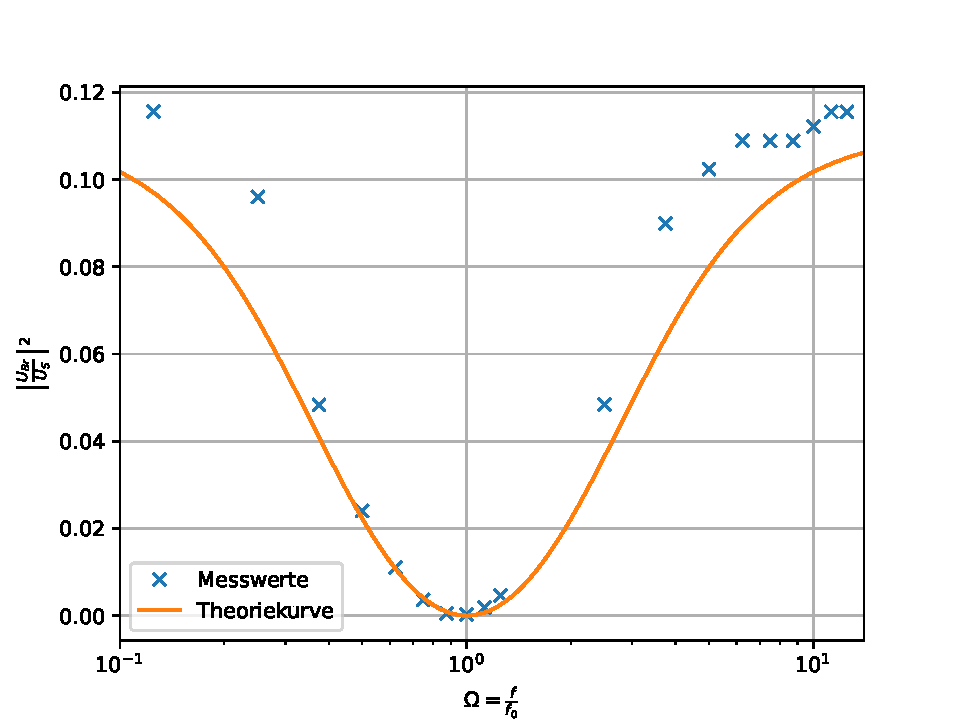
\includegraphics{plot.pdf}
  \caption{Halblogarithmische Darstellung der Frequenz und Spannung.}
  \label{fig:WienRobinson}
\end{figure}
\subsection{Klirrfaktor}
